\question \textbf{Matching - Application 2}

The 7 students $S_1, \dots , S_7$ of the Bioinformatics master program are looking for a supervisor.
There are the three professors Fox, Q, and Stark.
The students show their interest to work with certain professors as follows:\\
\textbf{Fox}: $S_2, S_3, S_4, S_6,$\\
\textbf{Q}: $S_1, S_3, S_5, S_7,$\\
\textbf{Stark}: $S_2, S_3$.\\

\begin{parts}

\part How many students can write a master thesis, if every professor accepts only one student? Model the problem as a bipartite graph and find a maximum matching in it.

\begin{solution}

    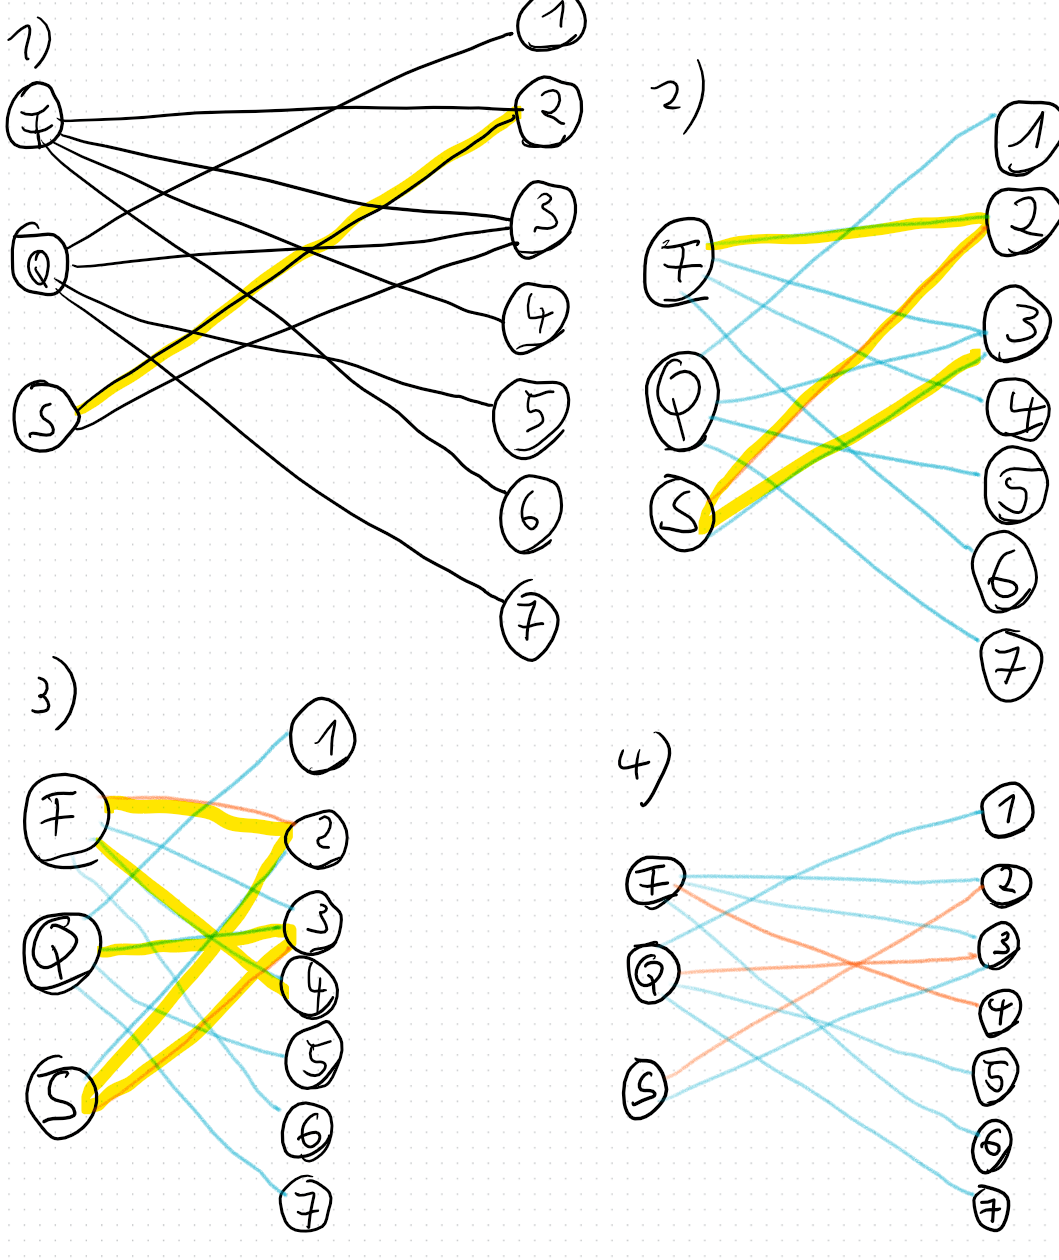
\includegraphics[width=0.7\linewidth]{task_03/sheet11_task3a.png}
\end{solution}

\part The president of the university, Dr. Mario, decided that Prof. Fox has to accept up to 2 students, Prof. Q up to 3 students and Prof. Stark up to 4 students. Show via flows in a network how each student can be assigned to a professor.


\begin{solution}
    Starting with the matching from the previous task.

    
    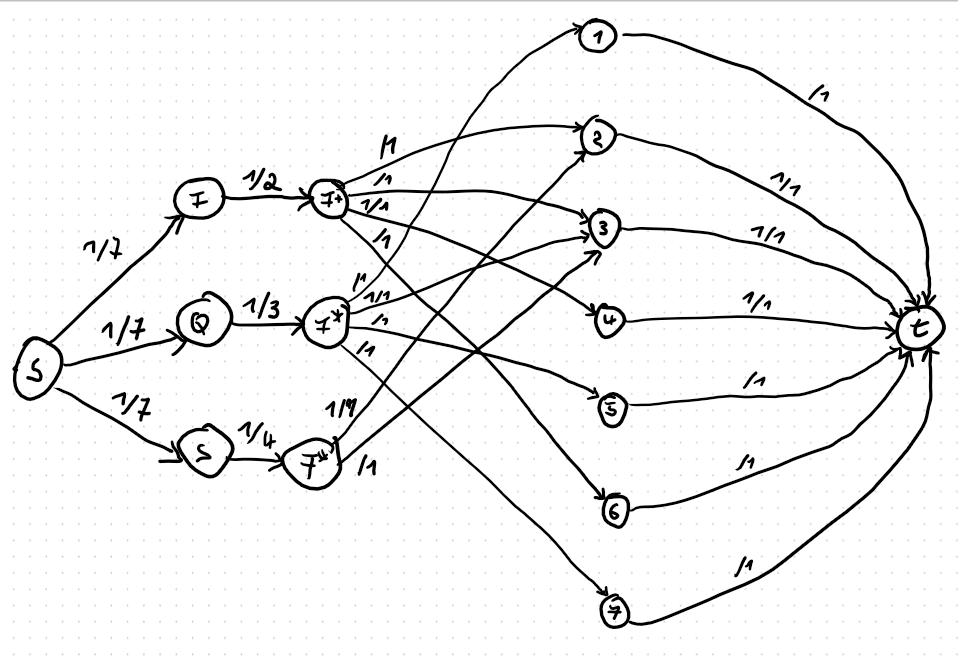
\includegraphics[width=0.5\linewidth]{task_03/sheet11_task3b_1.png}
    
    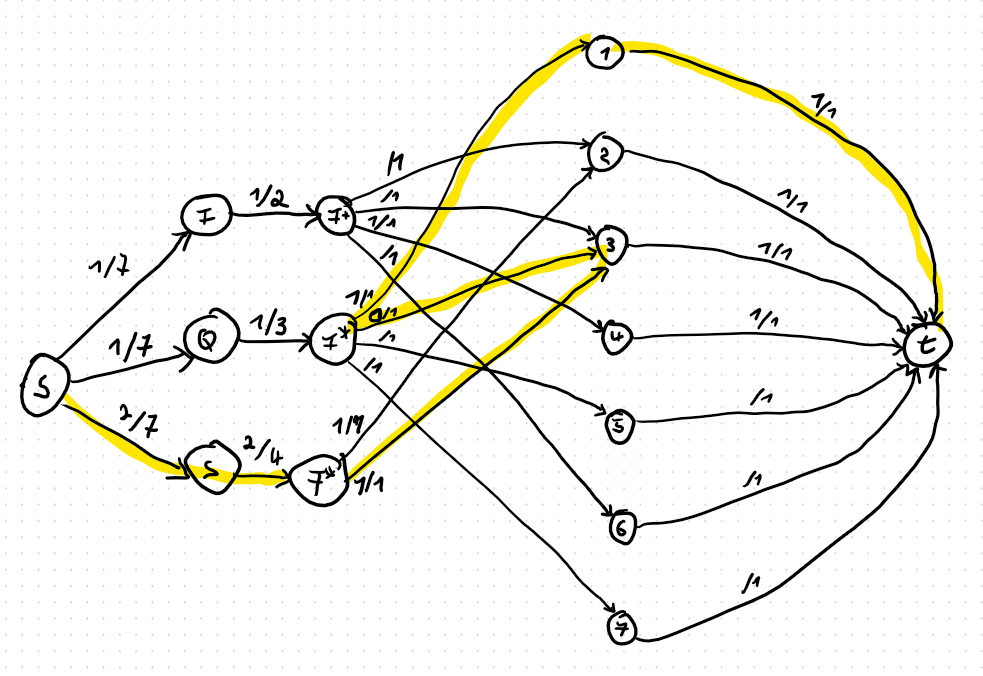
\includegraphics[width=0.5\linewidth]{task_03/sheet11_task3b_2.png}
    
    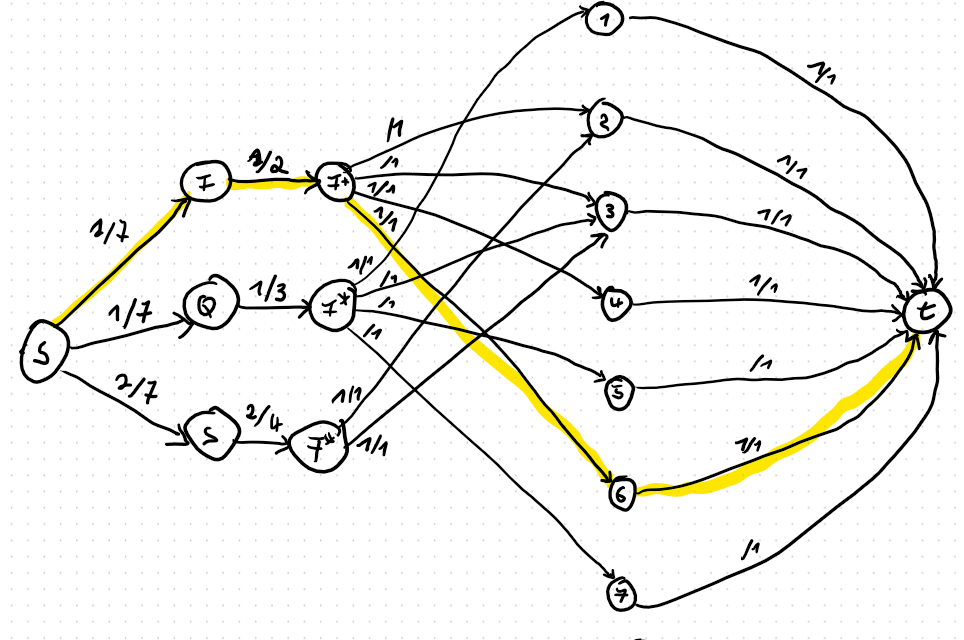
\includegraphics[width=0.5\linewidth]{task_03/sheet11_task3b_3.png}
    
    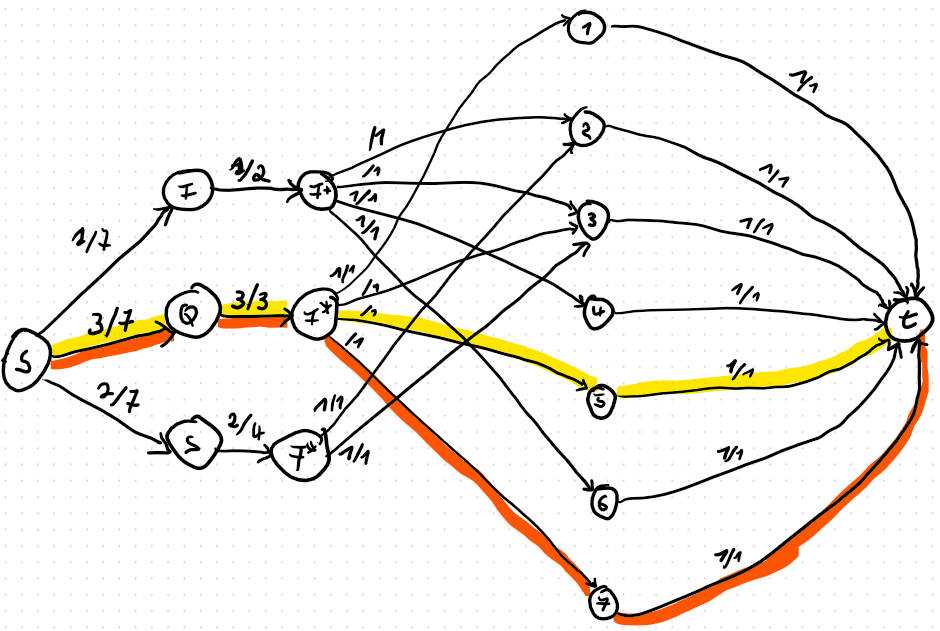
\includegraphics[width=0.5\linewidth]{task_03/sheet11_task3b_4.png}
    
    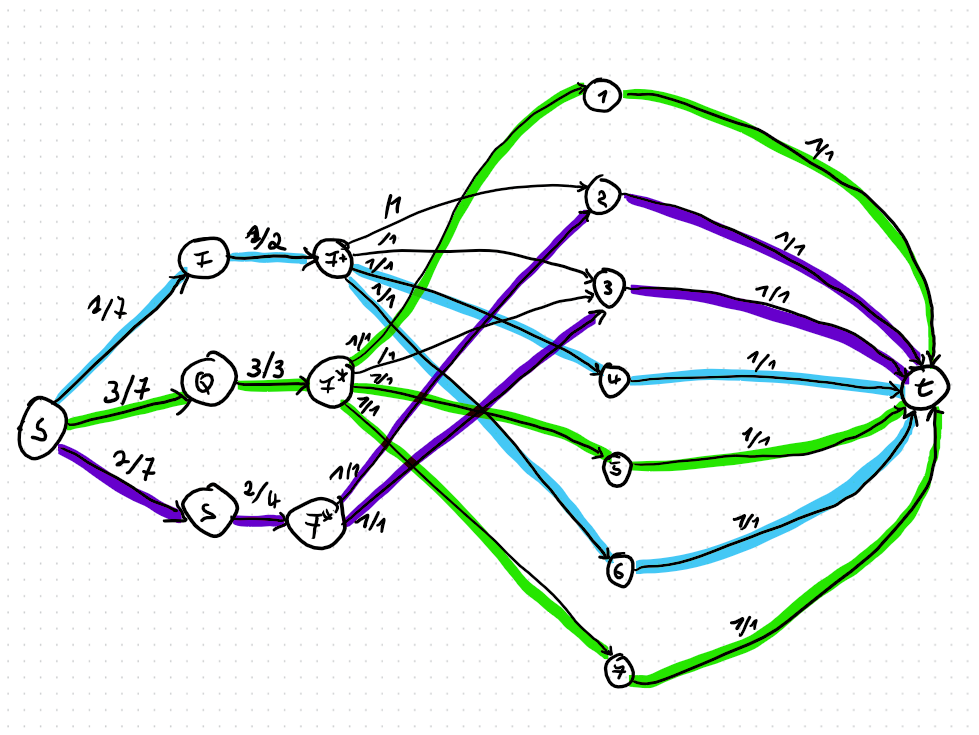
\includegraphics[width=0.5\linewidth]{task_03/sheet11_task3b_5.png}
\end{solution}

\end{parts}